\chapter{Introduction}\label{C:intro}

\section{Problem}\label{S:introproblem}

This project aims to verify the hypothesis that a new approach to representation learning should be able to generate a better general representation, despite only having access to noisy data. The project will explore this in a new extension to an existing state of the art in machine learning - the Restricted Boltzmann Machine. The new approach has been mathematically verified, but currently lacks reproducible, implemented tests to verify if the application matches the promise of the theory. Because this project sits as an extension to the Restricted Boltzmann Machine, this will be introduced in section \ref{S:introcontext}.

\section{Brief Context}\label{S:introcontext}
In recent years a new machine learning approach has risen in popularity - the use of stochastic, generative models. These are structures that can be trained to represent input data in a general way. Being generative, these structures try to recreate the input data based on the internal representation they have learnt, creating their own reconstructed version of the input data.
These structures, or 'machines' allow highly dimensional data, such as that of an image to be mapped to a much smaller and generalised representation.

One such system is a Restricted Boltzmann Machine, shortened to RBM. RBMs can form models of training data, by training a matrix of 'weights' that allow it to map a visible pattern, like an image, to an internal representation. RBMs perform well in practice, Hinton found that two RBMs layered on top of each other is enough to capture an excellent model for handwritten digits \cite{Hinton:2006dk}. These layered RBMs or 'Deep Belief Networks' hold the current best performance in several machine learning tasks. Handwritten digit classification is one of such tasks, as well as general image classification \cite{Bengio:2013bu}.

This can reap benefits in machine learning tasks such as classification - being able to take unlabelled data and label it. Another application of this technology is speech recognition, like that found in smartphone voice assistants \cite{Ling:2015by}.

\section{Solution}\label{S:introsolution}

An appropriate example problem is the Completely Automated  Public Turing Test to Tell Humans and Computers Apart. This is more commonly referred to as CAPTCHA and the more recent variant reCAPTCHA \cite{1_shet_2014}. Both are used online for preventing automatic spam on websites and in the case of reCAPTCHA actually helping to build labelled machine learning datasets. This technology features a series of digits/characters composed with images of noise, as shown in Fig \ref{F:modernCaptcha}.


\begin{figure}[]
\begin{center}
	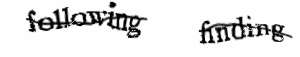
\includegraphics[]{Assets/Modern-captcha}
\caption{An example of a CAPTCHA, in this case a wobbly strikethrough obscures part of the text. \cite{pict} }
\label{F:modernCaptcha}
\end{center}
\end{figure}


CAPTCHA is analogous to real world image data in a sense it is not perfect, instead being noisy or containing more than one entity.
This project aims to verify the idea that if there are good models for two underlying causes, then they can each account for different parts of the image. This essentially means filtering so each model (RBM) can focus on the underlying, non-noisy entity.
The second outcome is, given only a noisy dataset,
the new approach can train two RBMs, one learning a model for the entity of interest and other modelling the noise. This separates the sources despite only seeing the noisy combination of them.

To achieve the aim of the project, the first goal is to gain enough understanding to extend the existing technology. This will be achieved by implementing the traditional RBM which can then be built on later with the new approach and provide a baseline to test from. The second goal is to implement a series of incremental tests, each increasing complexity of the data. These are to verify performance and therefore the tractability of this new approach and gain understanding of where the approach works. The tests also need to give insight that can help optimise this new approach as efficiency is definitely a risk that needs careful attention when it comes to working with these systems.

Finally, the tests should facilitate the project supervisor's ability to understand the problem and gain insight into the applications of the new approach.

\section{Scope Changes}\label{S:ScopeChanges}
The approach to testing (in a performance sense) of the the theory has been refined, with the size of the datasets and images that were being tested with, being reduced to evaluate a more atomic case. This increases understandability and has made it easier to judge what a correct output/performance is. Given the theory is untested in practice this reduces the risk by always ensuring that value is being added for the appropriate effort.

Also, the approach to evaluation has been altered as ongoing evaluation allows the author to incrementally 'tick off' the sizes and entities of datasets where the algorithm works.
As a result of these changes the updated Gantt Chart for this project is included  in fig \ref{F:gantt}
